% Статья: многокоординатная классификация распределённых SQL-СУБД.
% Шаблон: https://github.com/sadekovlar/misis-article-latex (файл misisarticle.cls должен лежать рядом).
% Компилятор: XeLaTeX (в CI — tectonic, см. .github/workflows/build.yml).
\documentclass{misisarticle}

\grnti{20.23.19}
\asjc{1710}
\oecd{1.2}

\title{Многокоординатная классификация распределённых SQL-СУБД: построение, проверка и применение к оценке надёжности}

% TODO(Viktor): добавь научного руководителя вторым \misisauthor при подаче и уточни почту.
\misisauthor{В.~Фокаиди}{кафедра инженерной кибернетики НИТУ «МИСиС»}{Москва, Россия}{viktorfokaidi@edu.misis.ru}

\setabstract{При проектировании информационных систем выбор распределённого SQL-хранилища и оценка его надёжности требуют классификации, из которой следуют предсказуемые архитектурные свойства; рыночные категории, такие как «NewSQL», этой задачи не решают. Предложена процедура построения и проверки многокоординатной классификации: определена мета-характеристика (архитектурные свойства, определяющие поведение системы при нагрузке и отказах); оси выведены из точек принятия решений эталонной архитектуры распределённой СУБД; корректность выбора проверена четырьмя исчислимыми тестами — релевантности, вариативности, проверяемости и независимости — и условиями завершения таксономии. Результат — классификация из семи осей (генезис распределённости, уровень её реализации, консенсус, глобальное упорядочивание транзакций, изоляция по умолчанию, движок хранения, интерфейсная совместимость) и архитектурные профили десяти систем. Проверка на выборке показала: все оси вариативны (нормированная энтропия 0,84–1,00); все значения профилей восстанавливаются из первичных источников; из 42 проверенных пар осей найдены три полные выборочные зависимости, каждая из которых разрушается реальными системами-контрпримерами (Galera, MySQL Group Replication, MyRocks, Oracle SERIALIZABLE, Snowflake) и потому является исторической ассоциацией, а не логической зависимостью. Построено отображение осей в классы сценариев отказов (RTO, RPO, деградация доступности и консистентности), превращающее вектор профиля в структурированный набор исходных данных для оценки надёжности на этапе проектирования.}
\setkeywords{многокоординатная классификация, распределённые SQL-СУБД, таксономия, NewSQL, архитектурный профиль, оценка надёжности.}

\begin{document}
\maketitle

\section{Введение и постановка задачи}

При проектировании прикладных информационных систем --- от процессных SCM-систем~\cite{levin} до технологий семантического быстрого поиска по специализированным БД~\cite{misissearch} --- архитектор выбирает хранилище до его реализации и оценивает его надёжность по косвенным данным: документации, публикациям, опыту эксплуатации. Такая оценка возможна только если классификация хранилищ, которой пользуется архитектор, обладает предсказательной силой: из класса или описания системы должны следовать её свойства при нагрузке и отказах. Стандартный инструмент рынка --- категория «NewSQL», введённая аналитиками в 2011~г.~\cite{aslett} и закрепившаяся в обзорной литературе~\cite{stonebraker2012,grolinger,sobol,oliveira} --- этой задачи не решает, и работа началась с проверки этого утверждения (раздел~2): рыночная категория оказалась не классом систем, а сегментом рынка, объединённым временем выхода продуктов и маркетинговым позиционированием.

\textbf{Постановка задачи.} Отрицание термина само по себе задачи классификации не решает: нужен конструктивный заменитель. Цель настоящей статьи --- \emph{построить многокоординатную классификацию распределённых SQL-СУБД и проверить её корректность}, а не только показать несостоятельность ярлыка. Вклад статьи:

\begin{itemize}
\item процедура построения и проверки классификации: определение мета-характеристики, конструктивный вывод осей из точек принятия решений эталонной архитектуры распределённой СУБД, четыре исчислимых проверочных теста и условия завершения таксономии (раздел~3);
\item результат процедуры --- классификация из семи осей и архитектурные профили десяти систем (разделы~3--4), включая статистическую проверку вариативности и независимости осей на выборке;
\item применение --- отображение осей в классы сценариев отказов, превращающее вектор профиля в структурированный набор исходных данных для оценки надёжности распределённых SQL-хранилищ на этапе проектирования (раздел~5).
\end{itemize}

Тем самым анализ термина «NewSQL» занимает в статье место мотивирующего случая --- примера категории, не прошедшей проверку, --- а содержательным результатом является сама классификация и метод её построения.

\section{Анализ работ: рыночная категория как ложный класс}

\subsection{Разграничение независимых признаков СУБД}

Следуя~\cite{elmasri}, будем называть \textbf{базой данных (БД)} организованную совокупность взаимосвязанных данных, а \textbf{системой управления базами данных (СУБД)} --- программную систему общего назначения, обеспечивающую определение, создание, манипулирование и совместное использование БД. \textbf{Реляционная модель данных}, предложенная Э.~Коддом~\cite{codd}, представляет БД как совокупность отношений --- множеств кортежей над заданными доменами.

Классификационные ошибки почти всегда порождаются смешением четырёх независимых признаков СУБД. Сам перечень требует обоснования, поэтому укажем, откуда каждый признак выводится и почему они независимы:

\begin{enumerate}
\item \textbf{модель данных} --- абстрактная структура представления данных (реляционная, документная, ключ-значение, графовая); это признак \emph{представления}, задаваемый теорией модели данных~\cite{codd,elmasri};
\item \textbf{интерфейс} --- язык доступа, предоставляемый приложению (диалект SQL, протокол совместимости, API); признак \emph{языка}, независимый от модели: одна модель реализуется разными языками, один язык --- поверх разных моделей (SQL поверх документной модели в Couchbase N1QL, SQL поверх реляционной в PostgreSQL);
\item \textbf{архитектура} --- способ организации вычислений и хранения (монолитная, распределённая shared-nothing, shared-disk, гибридная); признак \emph{реализации}, изучаемый теорией распределённых баз данных~\cite{ozsu}; один и тот же SQL-интерфейс существует и в монолитной, и в распределённой архитектуре;
\item \textbf{целевая нагрузка} --- класс рабочих задач (OLTP, OLAP, HTAP, поиск); признак \emph{назначения}, который, как показано Стоунбрейкером~\cite{stonebraker2005}, доминирует над архитектурой, но не выводится из неё.
\end{enumerate}

Независимость признаков следует из их комбинируемости: каждая пара значений реализуема --- реляционная модель с OLAP-нагрузкой (ClickHouse), документная модель с SQL-интерфейсом (Couchbase), реляционная модель с распределённой shared-nothing-архитектурой (PostgreSQL с Citus), документная модель с OLTP-нагрузкой (MongoDB). «NoSQL» объединяет под одним именем минимум три модели данных и даже не является утверждением о модели: изначально это было названием встречи сообщества в 2009~г. Категории каталога DB-Engines, при всей их полезности, также лежат на разных признаках: «RDF-хранилище» --- признак модели, «поисковая система» --- признак нагрузки, «многомодельная СУБД» --- признак реализации.

Важно и второе разграничение: \textbf{SQL-СУБД $\neq$ реляционная модель}. Ни одна промышленная SQL-СУБД, включая PostgreSQL, не реализует реляционную модель в строгом смысле: SQL допускает дубликаты кортежей (семантика мультимножеств), трёхзначную логику с NULL, значимый порядок атрибутов и таблицы без ключей --- расхождение между языком и моделью, подробно разобранное К.~Дейтом~\cite{date}. Название «NewSQL» указывает именно на язык интерфейса, то есть описывает систему по признаку, который вообще не разделяет системы между собой.

\subsection{Шесть проверяемых противоречий термина «NewSQL»}

Термин «NewSQL» возник в апреле 2011~г. в аналитическом материале М.~Аслетта~\cite{aslett} как рыночное наблюдение: на фоне успеха NoSQL появились продукты, «возвращающие» ACID и SQL в распределённом исполнении. Классификационным критерием изначально было \emph{время выхода продукта и маркетинговое позиционирование}, а не архитектура. Эта исходная слабость порождает каскад противоречий, каждое из которых проверяемо по открытым источникам.

\textbf{Противоречие~1. Класс включает архитектуры всех трёх возможных типов.} «NewSQL-подходы» делятся на «новые архитектуры», «оптимизированные движки хранения» и «прозрачное шардирование»~\cite{pavlo}: VoltDB --- распределённая in-memory система с процедурным исполнением, SingleStore --- гибридный row/column-движок, Vitess --- middleware над обычным MySQL. Общего архитектурного признака у них нет.

\textbf{Противоречие~2. В класс попадают технологии 1990-х и NoSQL-системы.} В вики-списки NewSQL входят MySQL Cluster (движок NDB, созданный Ericsson в 1990-х) и Couchbase --- документная NoSQL-СУБД, добавившая SQL-подобный язык N1QL. Если документная СУБД становится «реляционной NewSQL» за счёт SQL-подобного синтаксиса, граница класса утрачена.

\textbf{Противоречие~3. Системы, удовлетворяющие определению, в класс не попадают.} «Масштабируемость NoSQL + ACID + SQL» --- этому определению соответствует связка PostgreSQL + Citus~\cite{citus} и Vitess~\cite{vitess}, а также Oracle RAC (эксплуатируется с 2001~г.), IBM Db2 pureScale и Amazon Aurora с кворумным распределённым хранилищем~\cite{aurora} --- хотя архитектурно Aurora ближе к Spanner, чем VoltDB~\cite{spanner}.

\textbf{Противоречие~4. Флагман класса по исходному определению им не был.} Google Spanner --- образцовая NewSQL-система по вики-классификации --- на момент публикации описавшей её статьи~\cite{spanner} SQL-интерфейса не имел: язык запросов появился в 2015--2017~гг. Система вошла в «класс реляционных СУБД» до того, как стала поддерживать SQL.

\textbf{Противоречие~5. Члены класса нестабильны.} SingleStore сместилась к универсальной HTAP-платформе, VoltDB остался нишевой in-memory системой. Класс, определяемый по времени появления, размывается: системы «выходят» из него, не меняя архитектуру, --- меняется маркетинг.

\textbf{Противоречие~6. Каталоги и учебники класс не признают.} DB-Engines --- де-факто стандарт отраслевой систематики --- не содержит категории «NewSQL» и относит CockroachDB и Spanner к реляционным СУБД~\cite{dbengines}; фундаментальные учебники~\cite{elmasri,kleppmann} строят систематику по модели данных и архитектурным механизмам, не выделяя NewSQL. Термин удерживается в основном в обзорной и маркетинговой литературе~\cite{grolinger,sobol,oliveira}.

Из шести противоречий следует: «NewSQL» --- не класс, а \textbf{рыночный сегмент}. Как сегмент он описывает рынок; как классификация --- не описывает ничего: по ярлыку невозможно предсказать ни модель данных, ни архитектуру, ни гарантии, ни поведение при отказе. Для инженерной задачи (выбор хранилища, оценка надёжности) ярлык неинформативен, и каждая распределённая SQL-СУБД нуждается в описании, не зависящем от него. Конструированию такого описания и его проверке посвящены разделы~3--5.

\begin{figure*}[t]
\centering
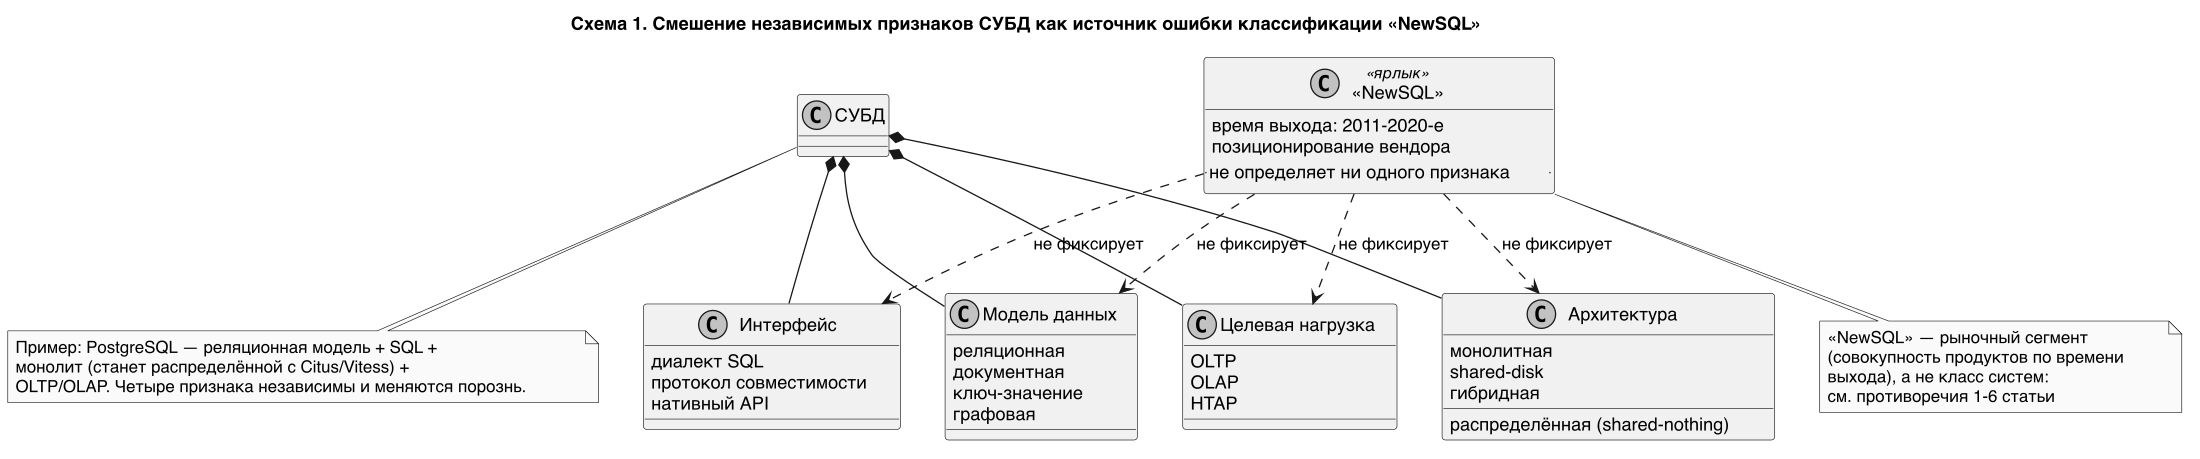
\includegraphics[width=0.92\textwidth]{figures/fig1.png}
\caption{Смешение независимых признаков СУБД как источник ошибки классификации «NewSQL»}
\label{fig:mix}
\end{figure*}

\section{Описание методов: построение и проверка классификации}

\subsection{Мета-характеристика и объект классификации}

Построение выполняется по методике разработки таксономий Ницкерсон, Варшни и Мунтерманна~\cite{nickerson}: классификация строится вокруг \textbf{мета-характеристики} --- свойства, ради описания которого таксономия создаётся, --- и признаётся завершённой при выполнении условий завершения (раздел~3.3). Использование формальной методики принципиально: она превращает выбор осей из перечисления в выводимую и проверяемую процедуру.

\textbf{Мета-характеристика} настоящей классификации: \emph{архитектурные свойства распределённой SQL-СУБД, определяющие её наблюдаемое поведение при нагрузке и отказах} --- то есть именно те данные, которые требуются для оценки надёжности на этапе проектирования. Мета-характеристика задаёт масштаб осей: ось включается не потому, что «есть такой признак», а потому, что её значения различают поведение систем.

\textbf{Объект классификации} --- распределённая SQL-СУБД: система, удовлетворяющая определению СУБД~\cite{elmasri}, предоставляющая приложению SQL-интерфейс (раздел~2.1) и хранящая данные более чем на одном вычислительном узле с распределением либо данных, либо обработки. Выборка для проверки строится по критерию: система упомянута как NewSQL в обзорах~\cite{aslett,pavlo,grolinger,oliveira} \emph{или} является распределённой SQL-СУБД по определению выше; выборка должна покрывать обе группы --- и «относимые к NewSQL», и явно не относимые (эволюционные системы), поскольку проверяемый тезис состоит в том, что граница между ними не является классификационной.

\subsection{Конструктивный вывод осей: точки принятия решений эталонной архитектуры}

Оси не перечисляются, а выводятся из эталонной архитектуры распределённой СУБД. Архитектура распределённой СУБД описывается как конвейер слоёв: приложение $\to$ интерфейсный уровень $\to$ координация транзакций $\to$ согласование реплик (репликация/консенсус) $\to$ уровень хранения; к конвейеру добавляются два внешних измерения --- уровень, \emph{на котором} реализована распределённость (по Кателлу~\cite{cattell}: middleware, нативное ядро, общий уровень хранения), и генезис системы --- история её разработки. Компонентный разбор СУБД, показавший, что подсистемы устаревают и переписываются независимо~\cite{endofera}, и структура компромиссов согласованность/задержка/доступность~\cite{abadi,bailis} указывают, в каких именно точках конвейера независимые проектные решения влияют на поведение при нагрузке и отказах.

Правило вывода оси: \textbf{осью становится точка конвейера (или внешнее измерение), в которой (а) эталонная архитектура допускает взаимно исключающие варианты реализации, (б) существующие системы в этих вариантах реально разошлись и (в) выбор варианта влияет на мета-характеристику}. Три условия устраняют произвол: точка, в которой все системы совпадают, не даёт оси (не выполняется (б)); точка, выбор в которой не влияет на поведение при отказах и нагрузке, не проходит (в). Применение правила к семи точкам даёт оси К1--К7 (табл.~\ref{tab:axes}).

\begin{table*}[t]
\caption{Оси классификации как точки принятия решений эталонной архитектуры}\label{tab:axes}
\centering
\small
\begin{tabular}{p{2.6cm}p{2.8cm}p{3.4cm}p{6.6cm}}
\toprule
\textbf{Ось} & \textbf{Точка эталонной архитектуры} & \textbf{Вопрос, на который отвечает} & \textbf{Типовые значения (домены)} \\
\midrule
К1. Генезис распределённости & внешнее измерение: история разработки & Система родилась распределённой или стала ею? & Э --- эволюционный путь (зрелая СУБД + средства распределения); Р --- революционный (распределённое ядро с нуля) \\
К2. Уровень реализации распределённости & все слои: где живёт распределённость & Какой компонент реализует распределение? & M --- middleware/прокси над узлами; N --- нативно в ядре; S --- общий уровень хранения (shared-disk, decoupled storage) \\
К3. Механизм репликации и консенсуса & слой согласования реплик & Как система согласует копии данных? & консенсус по партициям (Raft/Paxos); кворумное хранение; синхронная кластерная репликация; 2PC + репликация шардов; k-safety партиций \\
К4. Глобальное упорядочивание транзакций & слой координации транзакций & Откуда берётся глобальный порядок транзакций? & нет (локальный порядок/координатор); TrueTime; гибридные логические часы (HLC); централизованный сервис меток (TSO); порядок по партициям \\
К5. Уровень изоляции по умолчанию & интерфейс транзакционных гарантий & Какие аномалии допускает система «из коробки»? & read committed; repeatable read/SI; snapshot (внешне согласованный); serializable \\
К6. Движок хранения & слой хранения & Как данные физически организованы? & B-tree/heap; LSM; LSM + колонки; in-memory; log-structured; таблетки на распределённой ФС \\
К7. Интерфейсная совместимость & интерфейсный уровень & Чем система совместима для приложений? & PostgreSQL-протокол и диалект; MySQL-протокол и диалект; собственный диалект; несколько протоколов \\
\bottomrule
\end{tabular}
\end{table*}

Две точки конвейера, которые также удовлетворяют условию (а), не прошли условия (б): модель данных (в классе распределённых SQL-СУБД все системы реляционны) и целевая нагрузка (все системы позиционируются как транзакционные); их обсуждение вынесено в раздел~3.4. Модель развёртывания (self-hosted/DBaaS) не является точкой конвейера вовсе --- это коммерческая характеристика, и она в вектор не входит; для оценки надёжности решения она учитывается отдельным блоком исходных данных (раздел~5).

\subsection{Проверочные тесты: как проверить и как посчитать}

Выбор осей проверяется четырьмя независимыми тестами; каждый имеет определение, измеряемую процедуру и фиксируемый результат. Тесты не вложены друг в друга: каждый выполняется по своим данным.

\textbf{П1. Релевантность мета-характеристике.} Ось релевантна, если каждому её значению соответствует хотя бы один описанный в литературе класс сценариев отказа или нагрузочного поведения, и сценарные классы разных осей не совпадают. Измерение: построение отображения «ось $\to$ значение $\to$ класс сценариев $\to$ наблюдаемый показатель» (табл.~\ref{tab:faults}, раздел~5) и проверка его полноты. Результат: все семь осей отображены в различные классы сценариев (раздел~5); тест обусловлен субъективным условием завершения \emph{объяснимости}~\cite{nickerson}.

\textbf{П2. Вариативность.} Ось вариативна, если на выборке она принимает не менее двух значений из своего домена; иначе она не разделяет системы и осью не является. Измерение: число реализованных доменов значений, нормированная энтропия
\begin{equation}
H=\frac{-\sum_i p_i\log_2 p_i}{\log_2 k}
\end{equation}
и доля модального значения. Результат для выборки из 10 систем (раздел~4): все оси приняли от 2 до 6 доменов значений, $H=0{,}84$--$1{,}00$, доля моды не превышает 0,60 (табл.~\ref{tab:p2}). Тест связан с объективным условием завершения «нет пустых характеристик»~\cite{nickerson}: каждая характеристика каждого измерения реализована хотя бы одним объектом.

\textbf{П3. Проверяемость (воспроизводимость).} Каждое значение ячейки профиля должно восстанавливаться независимым исследователем из первичного источника --- научной публикации или официальной документации; маркетинговые заявления источником не признаются. Измерение: каждое из 70 значений профилей (10 систем $\times$ 7 осей, табл.~\ref{tab:profiles}) снабжено ссылкой на источник~\cite{spanner,crdb,tidb,aurora,citus,vitess,yugabyte,dbengines}; значения, допускающие неоднозначное прочтение, снабжены примечаниями. Тест соответствует объективному условию завершения «все объекты классифицированы» и требованию повторяемости~\cite{nickerson}. Заметим: ярлык «NewSQL» тест П3 не проходит в принципе --- его значение нельзя восстановить из первичных источников иначе, чем через дату выхода продукта.

\textbf{П4. Независимость (невыводимость).} Ось независима, если её значение не восстанавливается из значений остальных осей. Проверка двухчастная. \emph{Определительная часть}: определения осей ортогональны по построению --- каждая привязана к своему компоненту эталонной архитектуры, К1 --- к истории разработки, и ни одно определение не ссылается на значения других осей; это соответствует объективному условию завершения «каждое измерение уникально, дублирование измерений устраняется»~\cite{nickerson}. \emph{Исчислимая часть}: на выборке проверяются полные функциональные зависимости «значения оси $j$ $\Rightarrow$ значение оси $i$» по доменам значений --- всего 42 направленные пары. Найдены три полные зависимости (К3 $\Rightarrow$ К1, К4 $\Rightarrow$ К1, К5 $\Rightarrow$ К1): все системы с партиционным консенсусом, механизмами глобального порядка и повышенными уровнями изоляции по умолчанию --- революционного генезиса. Однако зависимость означает невыводимость только тогда, когда она \emph{логически необходима}, а для каждой из трёх существуют реальные системы-контрпримеры, разрушающие необходимость: Galera Cluster и MySQL Group Replication реализуют консенсусную репликацию с глобальным сертификационным порядком транзакций в эволюционной MySQL-инфраструктуре; Oracle поддерживает режим SERIALIZABLE (реализующий изоляцию уровнем выше read committed) с 1992~г.; CockroachDB, напротив, с версии 23.2 добавила режим read committed. Разрушены и более слабые ассоциации: Snowflake --- созданное с нуля распределённое SQL-ядро поверх отделяемого общего хранилища (К1 = Р при К2 = S, тогда как в выборке все Р-системы нативны), MyRocks --- LSM-движок в эволюционном MySQL (К6 = LSM при К1 = Э, тогда как в выборке LSM встречается только у Р-систем). Таким образом, ни одна из обнаруженных зависимостей и ассоциаций не является логической; они --- исторические закономерности выборки, которые сами по себе содержательны (раздел~4).

Суммарно процедура останавливается по условиям завершения~\cite{nickerson}: объективным --- все объекты выборки классифицированы полными векторами, пустых характеристик нет, дублирования измерений нет; субъективным --- \textbf{краткость} (число измерений 7 попадает в центр эмпирического диапазона 7$\pm$2, рекомендуемого как критерий удобства таксономии~\cite{nickerson} со ссылкой на Миллера), \textbf{устойчивость} (векторы различают системы: ни одна пара систем выборки не имеет одинаковых векторов), \textbf{полнота} (всякое новое проверяемое утверждение о системе выражается её вектором), \textbf{расширяемость} (добавление новой оси определено: кандидат обязан пройти П1--П4, раздел~3.4), \textbf{объяснимость} (П1: векторы объясняют поведение при отказах).

\subsection{Почему осей семь: отклонённые кандидаты и неприводимость}

Число осей --- не аксиома, а результат процедуры: применение правила раздела~3.2 к точкам эталонной архитектуры дало семь осей, прошедших тесты П1--П4. Существенно, что процедура определена и для отклонения кандидатов: каждый отклонённый кандидат снабжается номером проваленного теста (табл.~\ref{tab:rejected}). Именно этим отвечается на вопросы «почему не 6, не 8, не 10»: шесть осей означали бы слияние пары неприводимых осей (см. ниже), восемь --- включение кандидата, провалившего хотя бы один тест.

\begin{table}[t]
\caption{Кандидаты осей, отклонённые при проверке}\label{tab:rejected}
\centering
\footnotesize
\begin{tabular}{p{2.9cm}p{1.7cm}p{3.2cm}}
\toprule
\textbf{Кандидат-ось} & \textbf{Проваленный тест} & \textbf{Обоснование отклонения} \\
\midrule
Модель данных & П2 & константа в классе: все распределённые SQL-СУБД реляционны; нулевая энтропия \\
Целевая нагрузка (OLTP/OLAP/HTAP) & П2, П4 & константа в выборке; ортогональна архитектуре (TiDB: OLTP и OLAP на одних осях) \\
Модель согласованности (CAP/PACELC) & П4 & выводима из К3+К4+К5~\cite{abadi,bailis}; дублировала бы три оси \\
Модель развёртывания (self-hosted/DBaaS) & П1 & коммерческая характеристика, не точка архитектуры \\
Гео-топология кворумов & П2, П4 & параметр конфигурации, ограничивается К2--К3 \\
Лицензия, вендор, экосистема & П1 & не влияет на поведение при отказах и нагрузке \\
Наблюдаемость/телеметрия & П1 & влияет на диагностику, а не на классы отказов \\
Резервное копирование & П4 (не подтверждена) & релевантно (RPO при катастрофе), но коррелирует с К6; отложено до расширенной выборки \\
\bottomrule
\end{tabular}
\end{table}

Неприводимость проверяется с обеих сторон. \emph{Слияния}: объединение К3 и К4 в одну ось «транзакционный механизм» потеряло бы различение CockroachDB (Raft + HLC) и TiDB (Raft + TSO) --- систем, чья доступность записи при отказе координатора принципиально разная; объединение К2 и К3 стёрло бы различие между Aurora (кворум на уровне хранения) и MySQL Cluster (синхронная репликация в ядре). \emph{Расщепления}: выделение «модели согласованности» в восьмую ось избыточно --- она выводится из К3+К4+К5~\cite{abadi,bailis}. Гранулярность, таким образом, минимально достаточная: каждая ось --- одно независимое проектное решение, ни одно из которых не сводится к другим.

\begin{figure*}[t]
\centering
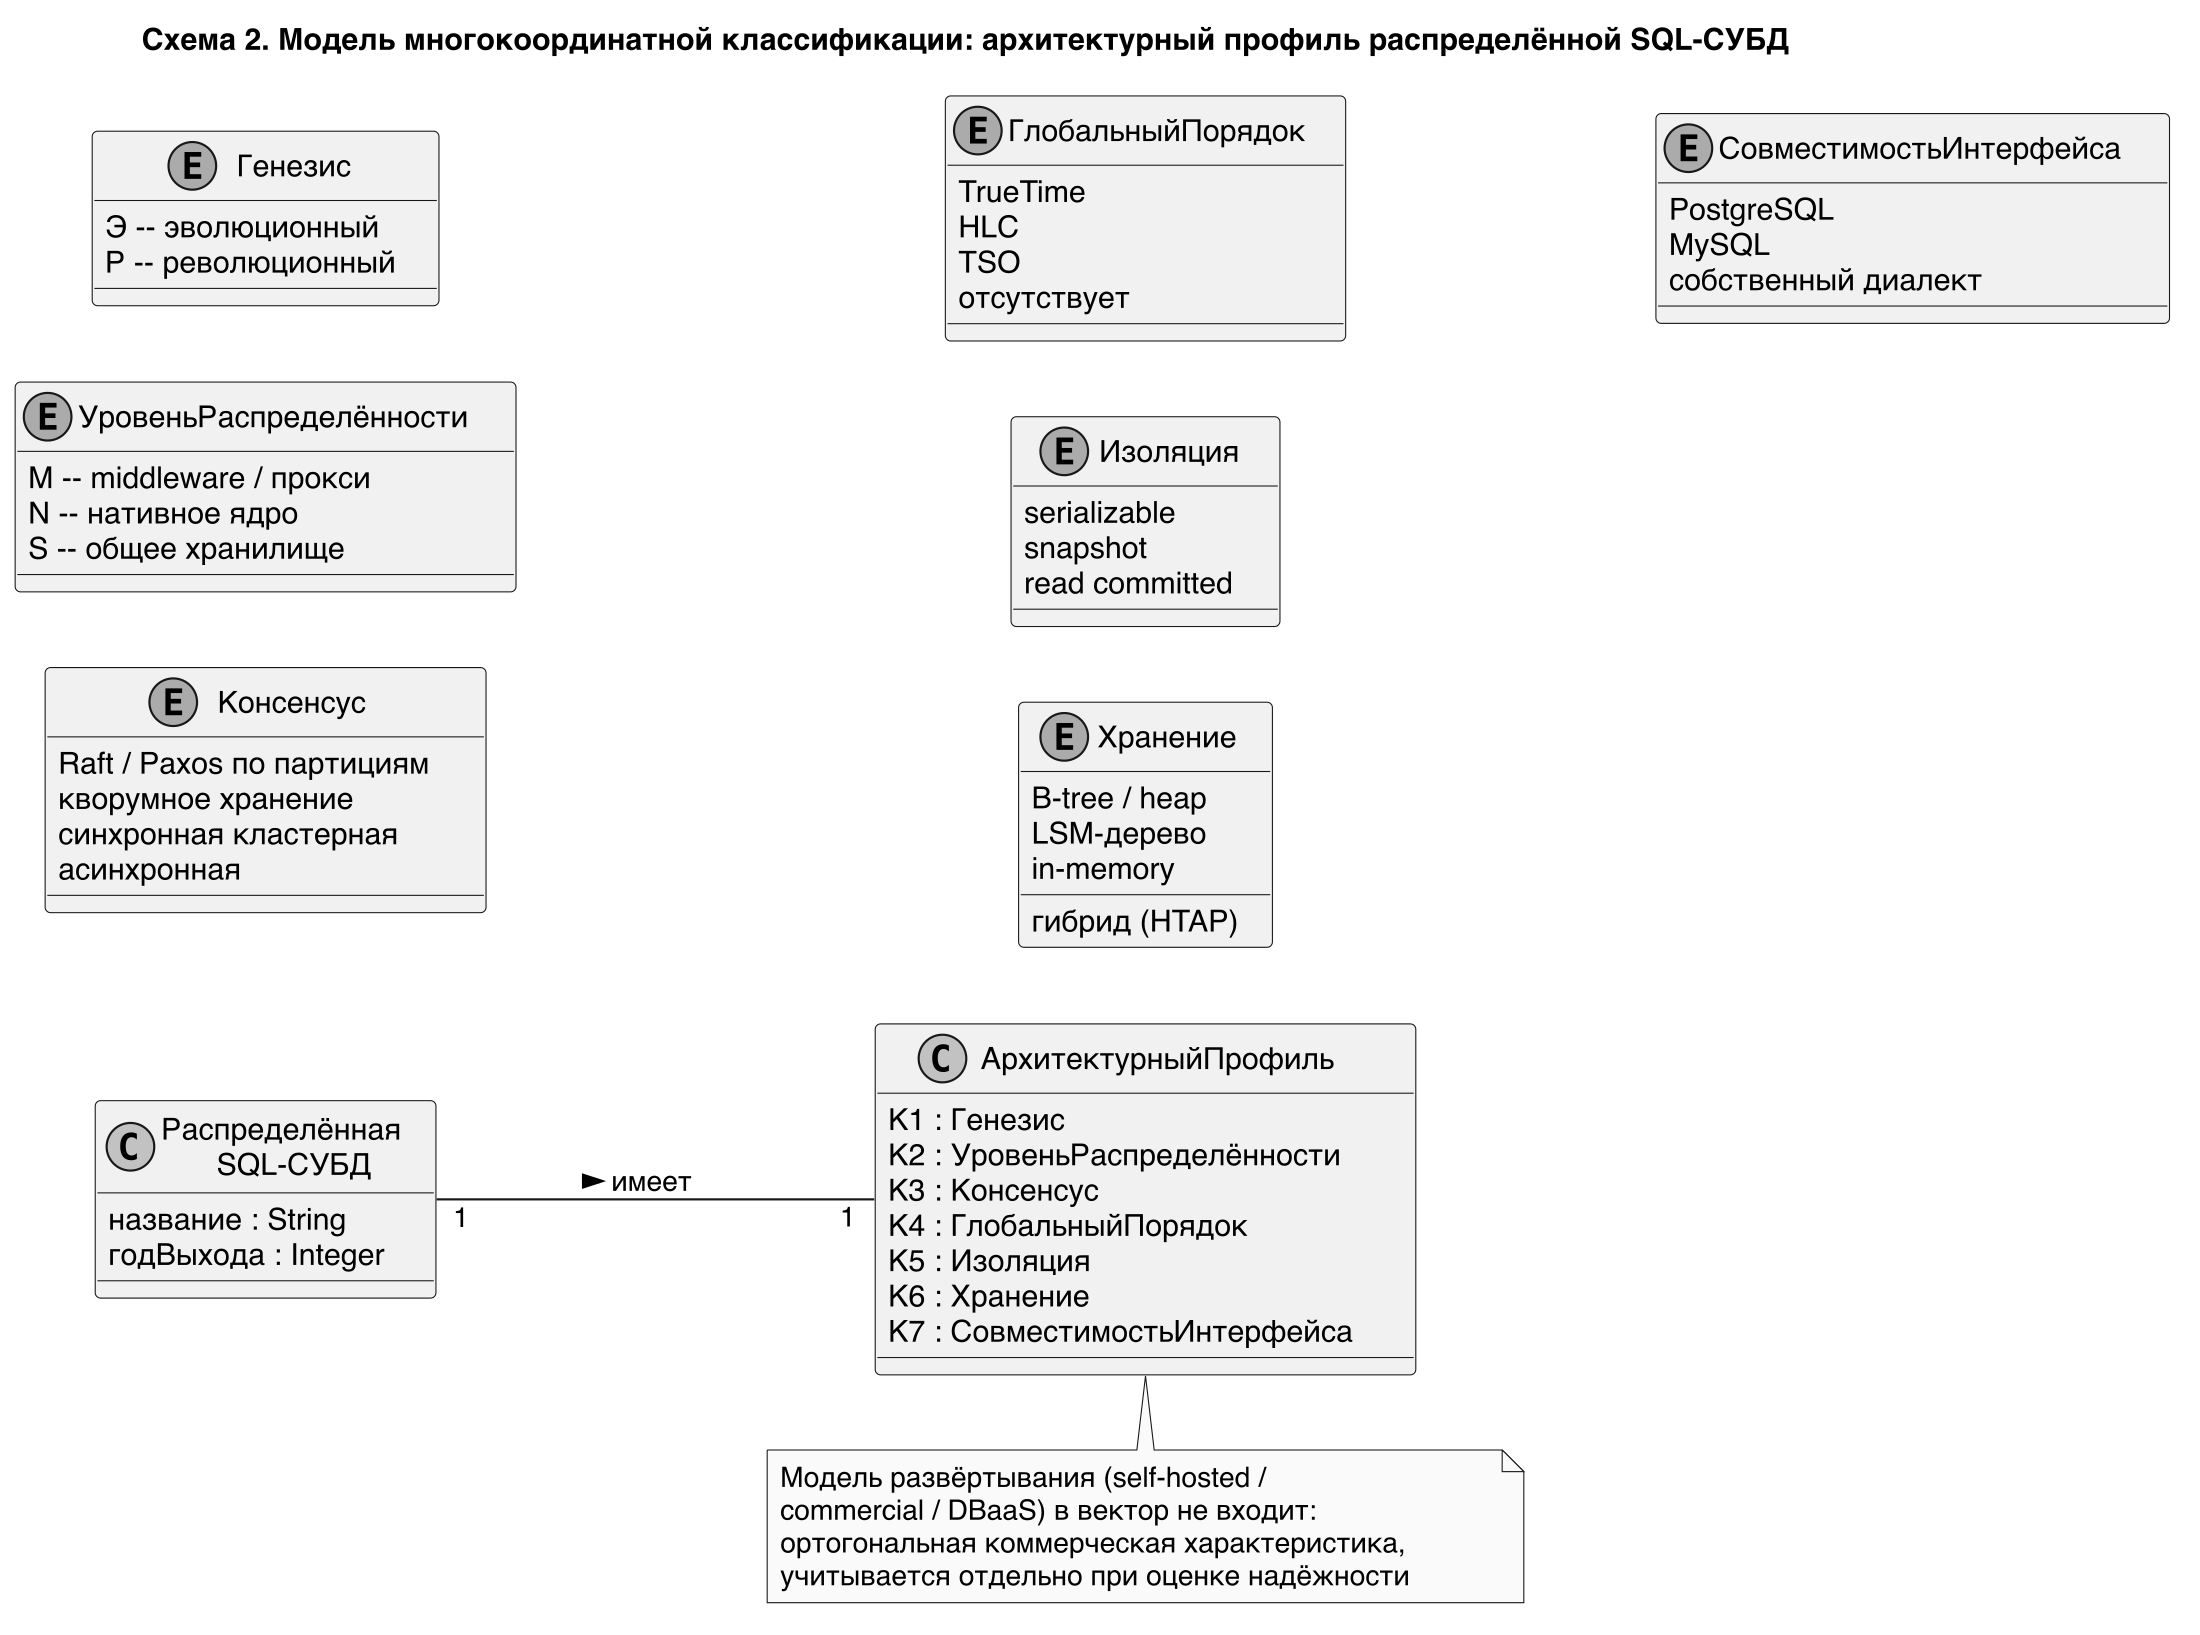
\includegraphics[width=0.85\textwidth]{figures/fig2.png}
\caption{Многокоординатная модель классификации: семь осей К1--К7}
\label{fig:model}
\end{figure*}

\section{Проверка на выборке: архитектурные профили десяти систем}

По осям К1--К7 построены профили десяти систем (табл.~\ref{tab:profiles}): пяти эволюционных (PostgreSQL + Citus, MySQL + Vitess, MySQL Cluster, Oracle RAC, Amazon Aurora) и пяти революционных (Google Spanner, CockroachDB, YugabyteDB, TiDB, VoltDB). Значения взяты из первичных публикаций~\cite{spanner,crdb,tidb,aurora} и официальной документации~\cite{citus,vitess,yugabyte}, дополненных каталогом DB-Engines~\cite{dbengines}; профили фиксируют состояние систем на 2026~г.; выбор значений проверяется тестом П3 (воспроизводимость из источников).

\begin{table*}[t]
\caption{Архитектурные профили распределённых SQL-СУБД}\label{tab:profiles}
\centering
\footnotesize
\begin{tabular}{llllllll}
\toprule
\textbf{Система} & \textbf{К1} & \textbf{К2} & \textbf{К3 (консенсус)} & \textbf{К4 (порядок)} & \textbf{К5 (изоляция)} & \textbf{К6 (хранение)} & \textbf{К7 (интерфейс)} \\
\midrule
PostgreSQL + Citus~\cite{citus} & Э & M & 2PC + репликация шардов & нет (координатор) & read committed & B-tree & PostgreSQL \\
MySQL + Vitess~\cite{vitess} & Э & M & 2PC + репликация шардов & нет & repeatable read$^{1}$ & B-tree & MySQL \\
MySQL Cluster (NDB) & Э & N & синхронная кластерная (NDB) & нет & read committed & in-memory + диск & MySQL-диалект \\
Oracle RAC & Э & S & Cache Fusion (shared-disk) & нет & read committed & B-tree & собственный \\
Amazon Aurora~\cite{aurora} & Э & S & кворум записи 4/6 по 3 зонам & нет (в зоне записи) & read committed (SI опц.) & log-structured storage & MySQL и PostgreSQL \\
Google Spanner~\cite{spanner} & Р & N & Paxos по сплитам & TrueTime (GPS + атомные часы) & snapshot (внешняя согласованность) & таблетки на Colossus & собственный (+ опц.\ PG) \\
CockroachDB~\cite{crdb} & Р & N & Raft по диапазонам & HLC & serializable (read committed опц.\ с 23.2) & LSM (Pebble) & PostgreSQL \\
YugabyteDB~\cite{yugabyte} & Р & N & Raft (DocDB) & HLC & snapshot (serializable опц.) & LSM (DocDB) & PostgreSQL \\
TiDB~\cite{tidb} & Р & N & Raft (TiKV) + кластер PD & TSO (Placement Driver) & snapshot (SI) & LSM (RocksDB) + колонки (TiFlash) & MySQL \\
VoltDB & Р & N & k-safety партиций & порядок по партициям & serializable & in-memory + снапшоты & собственный (процедурный) \\
\bottomrule
\end{tabular}

{\footnotesize $^{1}$\,Уровень изоляции по умолчанию в InnoDB --- repeatable read (семантически близок к snapshot isolation); в тесте П2 (табл.~\ref{tab:p2}) значение отнесено к домену «repeatable read/SI».}
\end{table*}

Результаты проверки на выборке.

\textbf{Полнота и различимость.} Все 70 ячеек профилей заполнены из первичных источников (П3); ни одна пара систем не имеет одинаковых векторов --- классификация различает все десять систем. Ближайшая пара --- CockroachDB и YugabyteDB --- совпадает по пяти осям и различается по К5 (serializable против snapshot): различие реально существует в документации обеих систем и воспроизводимо, то есть даже минимальное расстояние векторов несёт информацию.

\textbf{П2. Вариативность.} Все оси реально варьируют на выборке (табл.~\ref{tab:p2}): число реализованных доменов 2--6, нормированная энтропия 0,84--1,00, доля модального значения не выше 0,60. Ни одна ось не является константой --- в отличие от кандидатов «модель данных» и «нагрузка», чья энтропия в классе нулевая.

\begin{table}[t]
\caption{Результаты теста П2 (вариативность) на выборке десяти систем}\label{tab:p2}
\centering
\small
\begin{tabular}{lccc}
\toprule
\textbf{Ось} & \textbf{Доменов значений ($k$)} & \textbf{Нормированная энтропия} & \textbf{Доля моды} \\
\midrule
К1 & 2 & 1,00 & 0,50 \\
К2 & 3 & 0,87 & 0,60 \\
К3 & 5 & 0,91 & 0,40 \\
К4 & 5 & 0,85 & 0,50 \\
К5 & 4 & 0,92 & 0,40 \\
К6 & 6 & 0,95 & 0,30 \\
К7 & 4 & 0,95 & 0,30 \\
\bottomrule
\end{tabular}
\end{table}

\textbf{П4. Ассоциации осей как содержательный результат.} Исчислимая проверка независимости (раздел~3.3) обнаружила три полные выборочные зависимости (К3, К4, К5 $\Rightarrow$ К1) и ряд частичных ассоциаций: все революционные системы --- нативные (К2 = N) и с партиционным консенсусом; все эволюционные --- с 2PC/синхронной репликацией, B-tree-хранением и без глобального порядка (К4 = «нет»). Логической зависимости за ними нет (контрпримеры раздела~3.3), но как историческая закономерность наблюдение информативно: \textbf{«старые» и «новые» системы различаются не классом, а согласованным пучком независимых решений} по осям К2--К6. Это прямой ответ на исходный вопрос: то, что рынок называет «NewSQL», в векторном представлении распадается на комбинацию значений по независимым осям --- революционный генезис (К1) лишь статистически сопровождает этот пучок, а не определяет его.

Из векторного представления следуют и структурные наблюдения, недоступные ярлыку. CockroachDB, YugabyteDB и TiDB занимают практически одну ячейку пространства (Р/N/партиционный консенсус/LSM) и действительно конкурируют между собой; их реальные различия (TSO против HLC в К4, snapshot против serializable в К5, MySQL против PostgreSQL в К7) видны только в векторе. Профили PostgreSQL+Citus и MySQL+Vitess отличаются от «настоящих NewSQL» осями К1--К2, но совпадают с ними по остальным осям настолько же, насколько те совпадают между собой: эволюционный и революционный пути приводят в соседние точки пространства признаков, а не в разные классы. Amazon Aurora по осям К2--К7 ближе к Spanner, чем Spanner к VoltDB, --- однако первый «старый SQL», а вторые «один класс».

\begin{figure*}[t]
\centering
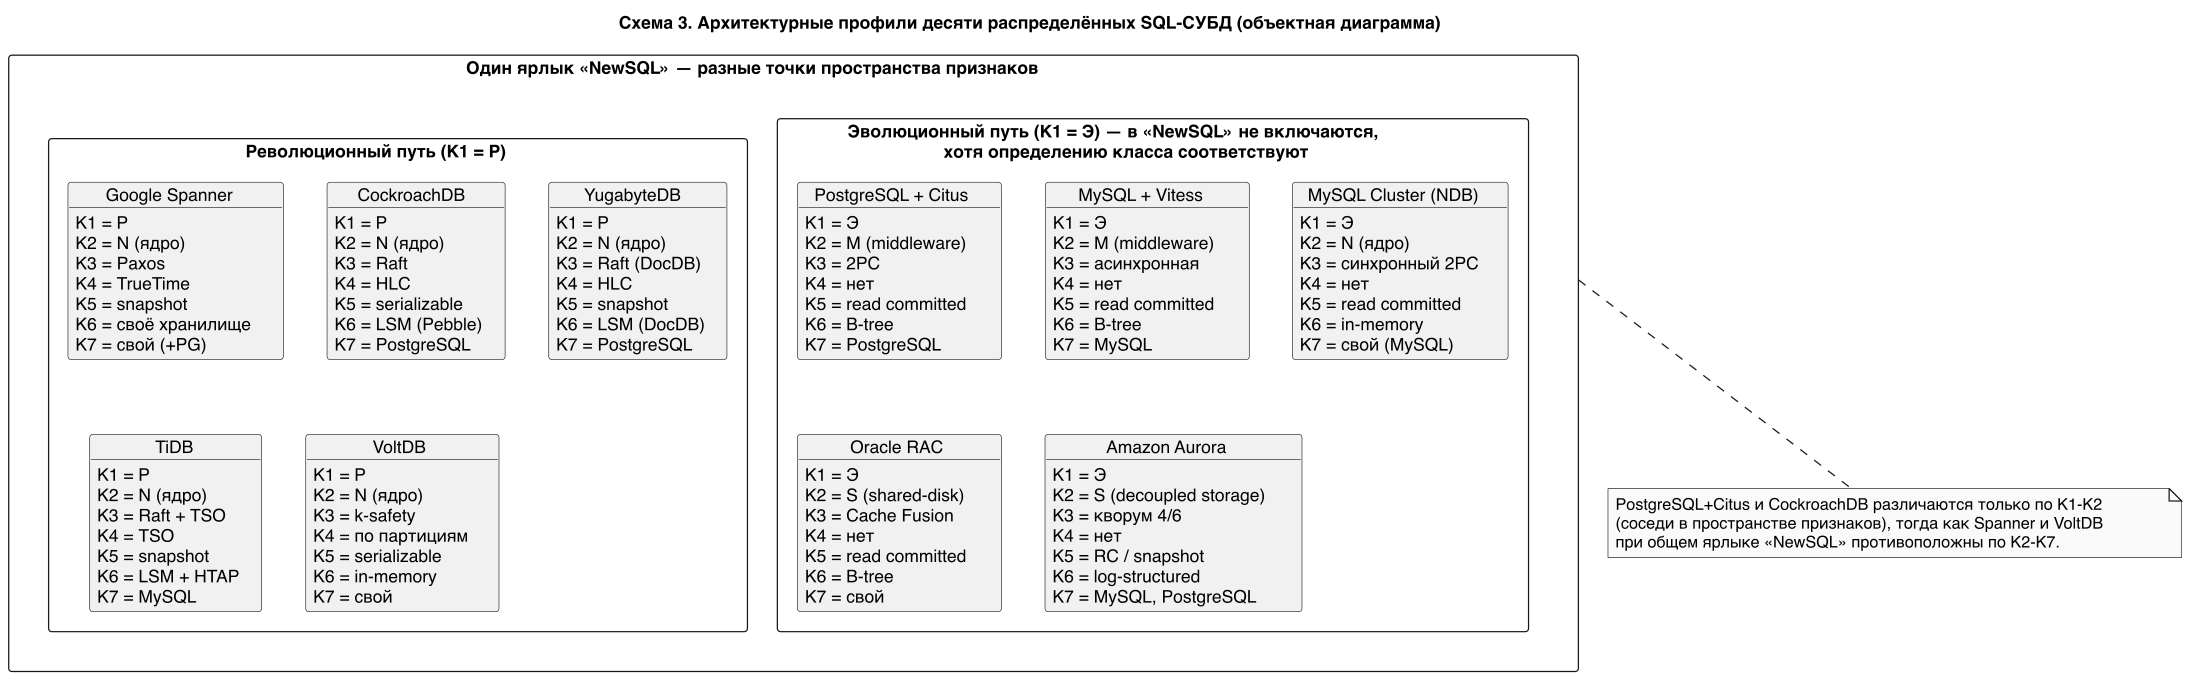
\includegraphics[width=0.92\textwidth]{figures/fig3.png}
\caption{Архитектурные профили десяти распределённых SQL-СУБД}
\label{fig:profiles}
\end{figure*}

\section{Применение: от осей к сценариям отказов и оценке надёжности}

Практическая ценность вектора в том, что каждая ось порождает свой класс сценариев отказов --- это одновременно проверка П1 (релевантность) и мост к оценке надёжности на этапе проектирования. Отображение «ось $\to$ значение $\to$ класс сценариев $\to$ наблюдаемый показатель» приведено в табл.~\ref{tab:faults}; сценарии опираются на первичные публикации систем~\cite{spanner,crdb,tidb,aurora,citus,vitess,yugabyte} и общую теорию распределённых систем~\cite{kleppmann,ozsu,abadi,bailis}.

\begin{table*}[t]
\caption{Отображение осей в классы сценариев отказов и наблюдаемые показатели}\label{tab:faults}
\centering
\footnotesize
\begin{tabular}{p{1.6cm}p{3.2cm}p{7.4cm}p{4.4cm}}
\toprule
\textbf{Ось} & \textbf{Значение} & \textbf{Класс сценариев отказов} & \textbf{Наблюдаемый показатель} \\
\midrule
К1 (генезис) & Э & граничные случаи поверх монолитного ядра (распределённые extension'ы не покрыты тестами исходной СУБД) & доля нештатных сценариев, требующих ручного разрешения \\
 & Р & производственная незрелость новых кодовых путей & частота дефектов ранних версий \\
К2 (уровень) & M & отказ координатора/маршрутизатора в контуре; подвешенные prepared-транзакции 2PC & RTO координатора; время ручного разрешения \\
 & N & протокольные режимы деградации (перевыборы лидера, переназначение диапазонов) & всплески задержки; доля недоступных партиций \\
 & S & концентрация риска в уровне хранения --- коррелированный отказ всех узлов & RTO/доступность уровня хранения \\
К3 (консенсус) & Raft/Paxos & отказ меньшинства копий --- доступность сохраняется; отказ большинства --- только чтение & порог кворума; RTO при потере кворума \\
 & кворумное хранение & порог перенесён на уровень хранения (запись 4/6) & допустимое число отказов узлов хранения \\
 & асинхронная репликация & расхождение копий, потеря данных при отказе & RPO $>$ 0 \\
 & 2PC & блокировка при отказе координатора между фазами & доля подвешенных транзакций \\
К4 (порядок) & TSO & недоступность сервиса меток останавливает распределённые транзакции & RTO сервиса меток \\
 & TrueTime & окно неопределённости (commit wait); зависимость корректности от физических часов & нижняя граница задержки коммита \\
 & HLC & нет централизации; осложнено разрешение конфликтов и внешняя согласованность & задержка разрешения конфликтов \\
 & нет & распределённые транзакции ограничены координатором & масштаб ограничений транзакций \\
К5 (изоляция) & serializable & аборты и рестарты при конфликтах & недетерминированность времени отклика \\
 & read committed & перенос риска аномалий на прикладной уровень & частота нарушений консистентности приложения \\
К6 (хранение) & LSM & фоновые компакции & хвосты задержки (P99) \\
 & in-memory & зависимость RPO от модели снапшотов и журналирования & RPO при катастрофическом отказе \\
К7 (интерфейс) & собственный диалект & уникальные кодовые пути --- меньше накопленных данных о надёжности & полнота данных об отказах \\
 & совместимость PG/MySQL & возможность канонических тестов надёжности и миграции & тестируемость, RTO миграции \\
\bottomrule
\end{tabular}
\end{table*}

Таким образом, вектор К1--К7 превращается в \textbf{структурированный набор исходных данных} методики оценки надёжности: характеристики топологии и репликации (К2, К3), транзакционных гарантий (К4, К5), механизмов восстановления (К6) и сопряжённых с ними сценариев отказов (отказ узла, отказ зоны доступности, отказ координатора/сервиса меток, потеря кворума, сетевой раздел). Сопоставление сценариев с нормативными требованиями заказчика (RTO, RPO, допустимая деградация консистентности) и с моделью развёртывания (учитываемой отдельным блоком, раздел~3.2) даёт профиль надёжности архитектуры ещё до её реализации --- что и требуется на этапе проектирования. Подробная формализация показателей и нормирование составляют предмет отдельной работы.

\begin{figure*}[t]
\centering
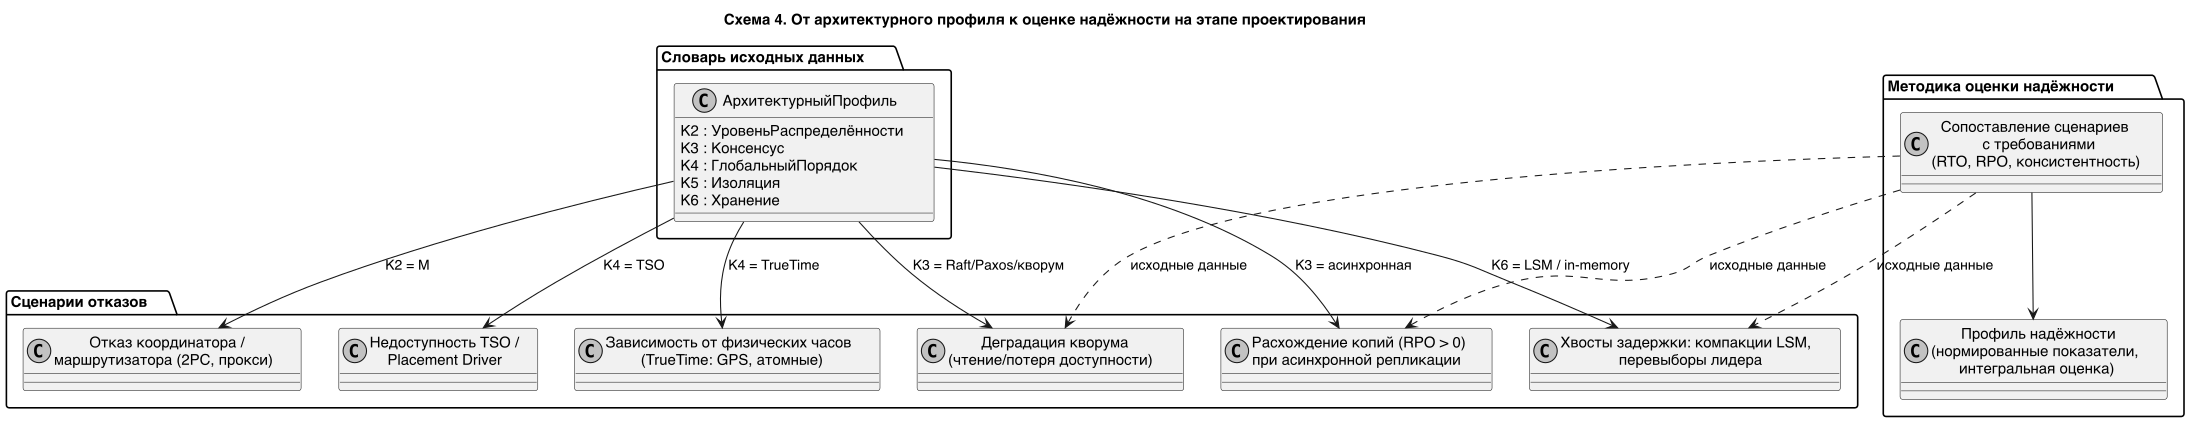
\includegraphics[width=0.85\textwidth]{figures/fig4.png}
\caption{От архитектурного профиля к оценке надёжности на этапе проектирования}
\label{fig:bridge}
\end{figure*}

\section{Заключение}

Предложена и проверена многокоординатная классификация распределённых SQL-СУБД вместе с процедурой её построения. Анализ термина «NewSQL» (раздел~2) выполнил роль мотивирующего случая: рыночная категория не проходит даже базовую проверку на класс (шесть проверяемых противоречий) и не может служить основой классификации.

Содержательные результаты:

\begin{itemize}
\item \textbf{процедура построения}: мета-характеристика (архитектурные свойства, определяющие поведение при нагрузке и отказах), конструктивный вывод осей из точек принятия решений эталонной архитектуры распределённой СУБД, четыре исчислимых проверочных теста (релевантность, вариативность, воспроизводимость, невыводимость) и условия завершения таксономии~\cite{nickerson};
\item \textbf{результат процедуры}: семиосевая классификация (генезис распределённости, уровень её реализации, консенсус, глобальное упорядочивание транзакций, изоляция по умолчанию, хранение, интерфейсная совместимость) и полные архитектурные профили десяти систем; выбор осей проверен измеримо: энтропия 0,84--1,00 по всем осям, воспроизводимость всех 70 значений из первичных источников, все три обнаруженные выборочные зависимости разрушены реальными контрпримерами (Galera, MySQL Group Replication, Oracle SERIALIZABLE, CockroachDB 23.2, MyRocks, Snowflake);
\item \textbf{содержательное наблюдение}: «старые» и «новые» системы различаются не классом, а согласованным пучком независимых решений по осям К2--К6 --- ярлык «NewSQL» распадается на комбинацию значений вектора;
\item \textbf{применение}: отображение осей в классы сценариев отказов (табл.~\ref{tab:faults}) делает вектор профиля словарём исходных признаков для оценки надёжности распределённых SQL-хранилищ на этапе проектирования.
\end{itemize}

Ограничения работы: выборка из десяти систем достаточна для проверки тестов, но не для окончательной оценки устойчивости ассоциаций; домены значений осей сгрубчены до категорий механизмов; ось «резервное копирование и восстановление» отложена как кандидат, не прошедший проверку независимости. Дальнейшая работа: расширение выборки и проверка кандидатов осей той же процедурой (резервное копирование, наблюдаемость); экспериментальная валидация методики оценки надёжности на архитектурах CockroachDB, YugabyteDB и Google Spanner; автоматизация построения профилей по документации.

\begin{thebibliography}{99}

\bibitem{codd} Codd E.~F. A Relational Model of Data for Large Shared Data Banks // Communications of the ACM. 1970. Vol.~13, No.~6. P.~377--387.

\bibitem{elmasri} Elmasri R., Navathe S.~B. Fundamentals of Database Systems. 7th ed. Boston: Pearson, 2016. 1200~p.

\bibitem{kleppmann} Клеппман М. Высоконагруженные приложения. Программирование, масштабирование, поддержка. СПб.: Питер, 2018. 640~с. (Kleppmann M. Designing Data-Intensive Applications. O'Reilly Media, 2017.)

\bibitem{aslett} Aslett M. How Will The Database Incumbents Respond To NoSQL And NewSQL? // The 451 Group. 2011. URL: \url{https://blogs.the451group.com/information_management/2011/04/15/nosql-newsql-and-beyond/} (дата обращения: 11.10.2026).

\bibitem{stonebraker2012} Stonebraker M. New Opportunities for New SQL // Communications of the ACM. 2012. Vol.~55, No.~11. P.~10.

\bibitem{pavlo} Pavlo A., Aslett M. What's Really New with NewSQL? // ACM SIGMOD Record. 2016. Vol.~45, No.~2. P.~45--55. DOI: 10.1145/3003665.3003674.

\bibitem{stonebraker2005} Stonebraker M., \c{C}etintemel U. ``One Size Fits All'': An Idea Whose Time Has Come and Gone // Proc. 21st International Conference on Data Engineering (ICDE). IEEE, 2005. P.~2--11.

\bibitem{spanner} Corbett J.~C. et al. Spanner: Google's Globally-Distributed Database // Proc. 10th USENIX Symposium on Operating Systems Design and Implementation (OSDI). 2012. P.~251--264.

\bibitem{crdb} Taft R. et al. CockroachDB: The Resilient Geo-Distributed SQL Database // Proc. ACM SIGMOD International Conference on Management of Data. 2020. P.~1493--1509.

\bibitem{tidb} Huang D. et al. TiDB: A Raft-based HTAP Database // Proceedings of the VLDB Endowment. 2020. Vol.~13, No.~12. P.~3072--3084.

\bibitem{aurora} Verbitski A. et al. Amazon Aurora: Design Considerations for High Throughput Cloud-Native Relational Databases // Proc. ACM SIGMOD International Conference on Management of Data. 2017. P.~1041--1052.

\bibitem{grolinger} Grolinger K. et al. Data Management in Cloud Environments: NoSQL and NewSQL Data Stores // Journal of Cloud Computing: Advances, Systems and Applications. 2013. Vol.~2, Art.~22.

\bibitem{sobol} Соболь А.~С. Построение и адаптация NewSQL СУБД в частном «облаке» // Актуальные проблемы авиации и космонавтики. 2013. Т.~14, №~4 (раздел «Информационные технологии»).

\bibitem{oliveira} Oliveira J., Bernardino J. NewSQL Databases: MemSQL and VoltDB Experimental Evaluation // Proc. 9th International Joint Conference on Knowledge Discovery, Knowledge Engineering and Knowledge Management (KEOD). SCITEPRESS, 2017. P.~276--281. DOI: 10.5220/0006518902760281.

\bibitem{dbengines} DB-Engines Ranking of Database Management Systems. URL: https://db-engines.com/en/ranking (дата обращения: 11.10.2026).

\bibitem{citus} Citus Data. Documentation: Distributed PostgreSQL. URL: https://docs.citusdata.com (дата обращения: 11.10.2026).

\bibitem{vitess} Vitess: Scalable MySQL Clustering. Documentation. URL: https://vitess.io/docs/ (дата обращения: 11.10.2026).

\bibitem{yugabyte} YugabyteDB Documentation. Architecture. URL: https://docs.yugabyte.com/stable/architecture/ (дата обращения: 11.10.2026).

\bibitem{levin} Левин А.~О. Исследование и разработка проекта процессной информационной системы управления цепями поставок (часть~1) // Корпоративные информационные системы. 2018. Вып.~3. URL: https://corpinfosys.ru/archive/2018/issue-3/104-2018-3-scm (дата обращения: 12.10.2026).

\bibitem{misissearch} МИСиС: Технология семантического быстрого поиска по специализированным базам данных // TAdviser --- портал о корпоративном и государственном ИТ. URL: https://www.tadviser.ru/index.php/Продукт:МИСиС:\_Технология\_семантического\_быстрого\_поиска\_по\_специализированным\_базам\_данных (дата обращения: 12.10.2026).

\bibitem{soloviev} Соловьев А.~В. [Название статьи --- заполнить по elibrary] // Электронная библиотека eLibrary.ru. URL: https://elibrary.ru/item.asp?id=91752646 (дата обращения: 12.10.2026).

\bibitem{ozsu} \"Ozsu M.~T., Valduriez P. Principles of Distributed Database Systems. 4th ed. Cham: Springer, 2020. 674~p.

\bibitem{cattell} Cattell R. Scalable SQL and NoSQL Data Stores // ACM SIGMOD Record. 2011. Vol.~39, No.~4. P.~12--27. DOI: 10.1145/1626215.1626219.

\bibitem{abadi} Abadi D.~J. Consistency Tradeoffs in Modern Distributed Database System Design: Cap Is Only Part of the Story // Computer. 2012. Vol.~45, No.~2. P.~37--44. DOI: 10.1109/MC.2012.33.

\bibitem{bailis} Bailis P., Davidson A., Fekete A. et al. Highly Available Transactions: Virtues and Limitations // Proceedings of the VLDB Endowment. 2013. Vol.~7, No.~3. P.~181--192.

\bibitem{nickerson} Nickerson R.~C., Varshney U., Muntermann J. A method for taxonomy development and its application in information systems // European Journal of Information Systems. 2013. Vol.~22, No.~3. P.~336--359. DOI: 10.1057/ejis.2012.26.

\bibitem{endofera} Stonebraker M., Madden S., Abadi D.~J. et al. The End of an Architectural Era (It's Time for a Complete Rewrite) // Proceedings of the 33rd International Conference on Very Large Data Bases (VLDB). 2007. P.~1150--1160.

\end{thebibliography}

\end{document}
